\documentclass{article}
\usepackage[T1]{fontenc}
\usepackage[utf8]{inputenc}

\usepackage{xspace}
\usepackage{graphicx}
\usepackage{amsmath}
\usepackage{amsfonts}
\usepackage{subfig}
\usepackage{fullpage}
\usepackage{url,paralist}
\usepackage{caption}
\usepackage{slashbox}

\author{Philip Pickering\\ \url{pgpick@gmx.at} \and Marco Eilers\\ \url{eilers.marco@googlemail.com} \and Thomas Bracht Laumann Jespersen\\ \url{ntl316@alumni.ku.dk}}
\title{Statistical Methods for Machine Learning\\ Assignment 2: Basic Learning Algorithms}
\date{}

\newcommand{\vect}[1]{\ensuremath{\boldsymbol{\mathbf{#1}}}\xspace}

%% For readability in question 1.3
\newcommand{\Target}{\vect{\mathsf{T}}}
\newcommand{\vPhi}{\vect{\Phi}}
\newcommand{\vw}{\vect{w}}
\newcommand{\Szero}{\vect{S}_0}
\newcommand{\mzero}{\vect{m}_0}
\newcommand{\target}{\vect{\mathsf{t}}}

\newcommand{\knollA}{\textsc{knollA}\xspace}
\newcommand{\knollB}{\textsc{knollB}\xspace}
\newcommand{\knollC}{\textsc{knollC}\xspace}

%% %% Uncomment these lines to get a box around all figures
%% \usepackage{float}
%% \floatstyle{boxed}
%% \restylefloat{figure}

\begin{document}
\maketitle

\section{Neural Networks}

\subsection{Neural Network implementation}

Implement a multi-layer neural network with linear output neuron and a
single hidden layer with non-linear neuron. All neurons should have
bias (offset) parameters.

To find the derivative of the activation function:
\[
\sigma(u) = \frac{|u|}{1 + |u|}
\]
we apply the quotient rule for differantiation:
\[
\frac{d}{du}\frac{f(x)}{g(x)} = \frac{g(x)f'(x) - g'(x)f(x)}{\left[g(x)\right]^2}
\]
where, in our case $f(u) = |u|$ and $g(u) = 1 + |u|$.
\begin{align}
  \frac{d}{du}\left(\frac{|u|}{1 + |u|}\right) &= \frac{(1 + |u|)\cdot 1 - (0 + 1)|u|}{(1 + |u|)^2}\\
  &= \frac{1 + |u| - |u|}{(1 + |u|)^2}\\
  &= \frac{1}{(1 + |u|)^2}
\end{align}

Implement backpropagation to compute gradient of error with respect to
the network parameters.

\subsection{Neural Network training}

Fig.~\ref{fig:semilognn} plots the $\frac{\sin{x}}{x}$ on the range $[-10,10]$ along with the predictions of our trained NN model.

\begin{figure}[!h]
  \centering
  \includegraphics[width=.8\textwidth]{semilognn.eps}
  \caption{Plot of $\frac{\sin{x}}{x}$ width neural network predictions for the same range.}
  \label{fig:semilognn}
\end{figure}

\newpage
\section{Support Vector Machines}

For this part of the assignment we chose to use the LIBSVM software.

\subsection{Model Selection}
Description (we normalized the data, then used the builtin function of libsvm, tried these values for gamma: [])

We did grid search using the following values of $\gamma: \{ 0.0001, 0.001, 0.01, 0.1, 1, 10, 100 \}$. This choice is based on what?

LIBSVM has built-in functionality to perform $n$-fold cross validation
given a command line option. To perform model selection we iterate
through all combinations of $C$ and $\gamma$ and call a function
called \texttt{crossval}, which invokes LIBSVM to perform a 5-fold
cross validation on the current values of $C$ and $\gamma$. When
performing $n$-fold cross validation, LIBSVM returns the accuracy,
which we  use to keep track of the configuration that gives the
highest accuracy.

\begin{table}[!h]
  \centering
  \begin{tabular}{l | c | c | c | c | c | c}
    \backslashbox{$\gamma$}{$C$} & $0.1$ & $1$ & $10$ & $100$ & $1000$ & $10000$\\\hline
    $0.0001$ & 55\% & 55\% & 55\% & 55\% & 55\% & 55\% \\
    $0.001$ & 55\% & 55\% & 55\% & 55\% & 55\% & 65\% \\
    $0.01$ & 55\% & 55\% & 56\% & 57\% & 65\% & 98\% \\
    $0.1$ & 60\% & 60\% & 59\% & 63\% & 98\% & 95\% \\
    $1$ & 57\% & 58\% & 59\% & 92\% & 97\% & 94\% \\
    $10$ & 51\% & 54\% & 67\% & 88\% & 92\% & 91\% \\
    $100$ & 52\% & 47\% & 76\% & 76\% & 77\% & 77\% \\
  \end{tabular}
  \caption{Table of all results for model selection using grid-search
    for \texttt{knollC-train100}.}
  \label{tab:crossval100}
\end{table}

\begin{table}[!h]
  \centering
  \begin{tabular}{l | c | c | c | c | c | c}
    \backslashbox{$\gamma$}{$C$} & $0.1$ & $1$ & $10$ & $100$ & $1000$ & $10000$\\\hline
    $0.0001$ & 55\% & 55\% & 55\% & 55\% & 55\% & 55\% \\
    $0.001$ & 55\% & 55\% & 55\% & 55\% & 55\% & 65\% \\
    $0.01$ & 55\% & 55\% & 56\% & 57\% & 65\% & 98\% \\
    $0.1$ & 60\% & 60\% & 59\% & 63\% & 98\% & 95\% \\
    $1$ & 57\% & 58\% & 59\% & 92\% & 97\% & 94\% \\
    $10$ & 51\% & 54\% & 67\% & 88\% & 92\% & 91\% \\
    $100$ & 52\% & 47\% & 76\% & 76\% & 77\% & 77\% \\
  \end{tabular}
  \caption{Table of all results for model selection using grid-search
    for \texttt{knollC-train200}.}
  \label{tab:crossval200}
\end{table}

\begin{table}[!h]
  \centering
  \begin{tabular}{l | c | c | c | c | c | c}
    \backslashbox{$\gamma$}{$C$} & $0.1$ & $1$ & $10$ & $100$ & $1000$ & $10000$\\\hline
    $0.0001$ & 55\% & 55\% & 55\% & 55\% & 55\% & 55\% \\
    $0.001$ & 55\% & 55\% & 55\% & 55\% & 55\% & 65\% \\
    $0.01$ & 55\% & 55\% & 56\% & 57\% & 65\% & 98\% \\
    $0.1$ & 60\% & 60\% & 59\% & 63\% & 98\% & 95\% \\
    $1$ & 57\% & 58\% & 59\% & 92\% & 97\% & 94\% \\
    $10$ & 51\% & 54\% & 67\% & 88\% & 92\% & 91\% \\
    $100$ & 52\% & 47\% & 76\% & 76\% & 77\% & 77\% \\
  \end{tabular}
  \caption{Table of all results for model selection using grid-search
    for \texttt{knollC-train400}.}
  \label{tab:crossval400}
\end{table}

%% Result: best parameters are:
%% C: 1000, gamma: 0.100000 Cross Validation Accuracy = 98%
%% C: 1000, gamma: 0.100000 Cross Validation Accuracy = 97.5%
%% C: 100, gamma: 1.000000 Cross Validation Accuracy = 97.5%
\begin{table}[!h]
  \centering
  \begin{tabular}{l | c | c | c }
    \hfill & $C$ & $\gamma$ & Acc.\\\hline
    \texttt{knollC-train100} & 1000 & 0.1 & 98\%\\
    \texttt{knollC-train200} & 1000 & 0.1 & 97.5\%\\
    \texttt{knollC-train400} & 100 & 1 & 97.5\%
  \end{tabular}
  \caption{Table of results for model selection using grid-search
    showing the optimal values for $C$ and $\gamma$.}
  \label{tab:svmoptimal}
\end{table}

Applied to the testdata, this gives the results in table ~\ref{tab:crossval100} to ~\ref{tab:crossval400}. The resulting optimal parameter configurations are shown in table ~\ref{tab:svmoptimal}.

\begin{table}[!h]
  \centering
  \begin{tabular}{l | c | c | c | c}
    \backslashbox{Model}{Data} & \texttt{knollC-train100} & \texttt{knollC-train200} & \texttt{knollC-train400} & \texttt{knollC-test}\\\hline
    \texttt{knollC-train100} & 98\% & 97.5\% & 96.75\% & 97\%\\
    \texttt{knollC-train200} & 98\% & 98\% & 97.5\% & 98\%\\
    \texttt{knollC-train400} & 99\% & 98.5\% & 97.25\% & 98\%
  \end{tabular}
  \caption{Percentage of correct predictions when applying the model from each training data set to the training and test data.}
  \label{tab:svmpredictresults}
\end{table}



\subsection{Inspecting the kernel expansion}

\subsubsection{Visualization}

Fig.~\ref{fig:freebounded} shows the plot of the \texttt{knollC-train200} data set, in which the support vectors are circled. The free support vectors are circled in black, and bounded are circled in green. There are 87 bounded support vectors, and just six free for a total of 93 support vectors.

\begin{figure}[!ht]
  \centering
  \includegraphics[width=.8\textwidth]{Code/freeBoundedSVs.eps}
  \caption{\texttt{knollC-train200} data set with free support vectors (circles) and bounded support vectors (squares).}
  \label{fig:freebounded}
\end{figure}

\subsubsection{Effect of the regularization parameter}

%%Retrain model on \texttt{knollC-train200} using values of $C$ that are 100 times larger and 100 times smaller than the $C*$ found during model selection. How does it change?

The file \texttt{regularization.m} performs the outlined procedure, by first training the SVM model using the values for $C$ and $\gamma$ found during model selection. Then it trains to other models, one in which $C$ is multiplied by a hundred and one in which we divide $C$ by 100.

The most notable change is in the number of support vectors. There's a total of 93 support vectors for the ``original'' value of $C$---87 of which are bounded. When $C$ is a hundred times larger, the number of support vectors drop to just 19, all of which are free. Conversely, when dividing $C$ by a hundred we get an increase in the number of support vectors to 199, but again all of them are free.

\subsubsection{Scaling behaviour}

Table of free and bounded 

\begin{table}[h!]
  \centering
  \begin{tabular}{l | c | c}
    \hfill & bounded & free\\\hline
    \texttt{knollC-train100} & 5 & 60 \\
    \texttt{knollC-train200} & 6 & 87 \\
    \texttt{knollC-train400} & 12 & 153 \\
  \end{tabular}
  \caption{Table of bounded and free support vectors for the three data sets.}
  \label{tab:knoll_free_bounded_SV}
\end{table}

\end{document}
